\chapter{Introduction}

Discovering the objective of an agent based on observations of its behavior is a problem that 
has interested both artificial intelligence (AI) and psychology researchers for many years \cite{schmidt:78,kautz:87}. 
In AI, this problem is known as \emph{goal recognition} (GR) or, more generally, \emph{plan recognition}~\cite{Sukthankar:14}. 
Plan and goal recognition problems have been used to model a number of applications ranging from software personal assistants~\cite{oh:10,oh:11,oh:11b}; 
robots that interact with humans in social settings such as homes, offices, and hospitals~\cite{tavakkoli:07,kelley:12}; 
intelligent tutoring systems that recognize sources of confusion or misunderstanding in students through 
their interactions with the system~\cite{mcquiggan:08,johnson:10,lee:12,min:14}; and security applications that recognize the plan or goal of terrorists~\cite{jarvis:05}. 


\begin{figure}[h!]
\begin{center}

  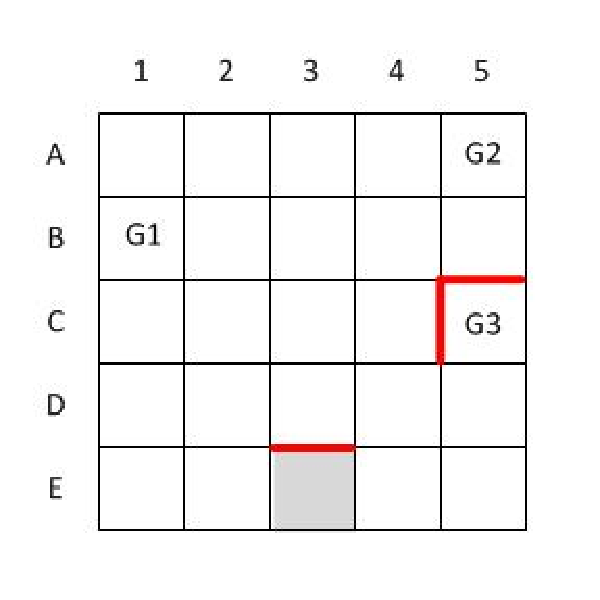
\includegraphics[scale=.15]{blocked}
  \end{center}

  \caption{Example Problem (left) and with Blocked Actions in Red (right).}
  \label{fig:blocked}
\end{figure}

One can broadly summarize the existing research in GR as one that primarily focuses on developing better and more 
efficient techniques to recognize the plan or the goal of the user given a sequence of observations of the user's actions. For example, imagine a %simplistic security 
scenario shown in Figure~\ref{example} (left), where an agent %(e.g.,~a potential terrorist) 
is at cell $E3$, it can move in any of the four cardinal directions, and its goal is one of three possible goals G1 (in cell $B1$), G2 (in cell $A5$), and G3 (in cell $C5$). Additionally, assume that it will move along a shortest path to its goal. Then, if it moves left to cell $E2$, then we can deduce that its goal is G1. Similarly, if it moves right to cell $E4$, then its goal is either G2 or G3. 

Existing research has focused on agent GR models that are non-strategic or
partially strategic: The agent's objective is to reach its goal with minimum cost, 
and the agent does not explicitly reason about its interaction with the observer.
However, when the observer's recognition of the agent's goal affects the agent in some way, 
then it is in the agent's best interest to be \emph{fully strategic} -- to \emph{explicitly} 
reason about how the agent's choice affects the observer's recognition. 
As a result, the observer will need to take into account the agent's strategic reasoning when making decisions.

\subsection{Game-Theoretic Goal Recognition Problems in Security Domains}
Naturally, GT settings with strategic agents are common in 
many real-world (physical and cyber) security scenarios between 
an adversary and a defender. 
The adversary has a set of targets of interests 
and would be equally happy in attacking one of them. 
In physical security domains, the adversary 
must make a sequence of 
physical movements to reach a target; 
in cyber security domains, this could be a sequence of 
actions achieving necessary subgoals to carry out the attack. 
In any case, the defender is trying to recognize
the adversary's goal/target. 
We coined this the game-theoretic goal recognition (GTGR) problem. 

Let us describe the security games of interests using Figure \ref{example}. 
Consider the security scenario in Figure \ref{example} (left),
where an agent (i.e., terrorist) wants to reach its intended target and carry out an attack, 
while we, the observer (the defender) try to recognize the agent's goal as early as possible. 
Suppose once we recognize the agent's goal, we will strengthen the agent's target to defend against the attack. 
The more time we have between recognition and the actual attack, the less successful the attack will be. 
In this scenario, it is no longer optimal for the agent to simply choose a shortest path to its goal, 
as that could allow the observer to quickly identify its goal. 
On the other hand, the agent still wants to reach its goal in a reasonably short time, 
as a very long path could allow the observer time to strengthen all the targets.
So, an optimal agent would need to explicitly reason about the tradeoffs 
between the cost of its path (e.g., path length) and the cost of being discovered early.

\subsection{Game-Theoretic Goal Recognition Design Problems in Security Domains}
So far we have been discussing the defender's task on recognizing goals. 
However, the task could become very difficult in general. 
For instance, going back to our security example in Figure \ref{example}, 
if the agent moves up to $D3$, the observer cannot make any informed deductions. 
In fact, if the agent moves along any one of its shortest paths to goal G3, 
throughout its entire path, which is of length 4, we cannot deduce whether its goal is either G2 or G3! 
This illustrates one of the challenges with this approach, that is, there are often a large number of 
ambiguous observations that can be a result of a large number of goals. 
As such, it is difficult to uniquely determine the goal of the agent until a long sequence of observations is observed.

The work of \cite{keren:14,keren:15} proposed an orthogonal 
approach to \emph{modify the underlying environment of the agent}, in such a way that 
\emph{the agent is forced to reveal its goal as early as possible}. 
They call this problem the goal recognition design (GRD) problem. 
For example, if we block the actions $(E3, up), (C4, right)$, $(C5, up)$ in our example problem, 
where we use tuples $(s,a)$ to denote that action $a$ is blocked from cell $s$, then the agent can 
make at most 2 actions (i.e.,~right to E4 then up to D4) before its goal is conclusively revealed. 
Figure~\ref{example} (right) shows the blocked actions. 
This problem finds itself relevant in many of the same 
applications of GR because, typically, the underlying environment can be easily modified. 

%(perhaps with the help of roadblocks as in Figure \ref{example} (right)).
As such, in addition to studying the GTGR problem, we consider the GTGRD problem 
where the observer can modify the underlying environment (i.e., adding $K$ roadblocks)
as to restrict the actions of the agent. 

\subsection{Related Work}

GR and its more general forms, plan recognition and intent recognition, have been extensively studied~\cite{Sukthankar:14} since their inception almost 40 years ago~\cite{schmidt:78}. Researchers have made significant progress within the last decade through synergistic integrations of techniques ranging from natural language processing~\cite{vilain:90,geib:07} to classical planning~\cite{ramirez:09,ramirez:10,ramirez:11} and deep learning~\cite{min:14}. The closest body of work to ours is the one that uses game-theoretic formulations, including an adversarial plan recognition model that is defined as an imperfect information two-player zero-sum game in extensive form~\cite{lisy:12}, 
a model where the game is over attack graphs~\cite{braynov:06}, 
and an extension that allows for stochastic action outcomes~\cite{guillarme:15}. 
The main difference between these works and ours is that ours focuses on goal recognition instead of plan recognition. 

While GR has a long history and extensive literature, the field of GRD is relatively new. Keren \emph{et al.} introduced the problem in their seminal paper~\cite{keren:14}, where they proposed a decision-theoretic STRIPS-based formulation of the problem. In the original GRD problem, the authors make several simplifying assumptions: (1) the observed agent is assumed to execute an optimal (i.e.,~cost-minimal) plan to its goal; (2) the actions of the agent are deterministic; and (3) the actions of the agent are fully observable. Since then, these assumptions have been independently relaxed, where agents can now execute boundedly-suboptimal plans~\cite{keren:15}, actions of the agents can be stochastic~\cite{wayllace:16}, and actions of the agents can be only partially observable~\cite{keren:16}. Further, aside from all the decision-theoretic approaches above, researchers have also modeled and solved the original GRD problem using answer set programming~\cite{son:16}. The key difference between these works and ours is that ours introduced a game-theoretic formulation that can more accurately capture interactions between the observed agent and the observer in security applications.  

\subsection{Our Contributions}
As a result of the strategic interaction in the GTGR and GTGRD scenarios, the concept of cost-minimal plan (the solution concept in GR problem) 
and worst-case distinctiveness (the solution concept in GRD problem)
are no longer a suitable solution concept since it does not reflect the behavior of strategic agents.
Instead, our objective here is to formulate game-theoretic models of the agent's and observer's interactions 
under GR and GRD settings. 
More specifically, we propose to model GTGR and GRGRD settings as zero-sum stochastic games
with incomplete information where the adversary's target is unknown to the observer. 
%We propose to model GTGR and GRGRD settings as zero-sum stochastic games
%with incomplete information about the adversary's intended target. %(i.e., private information).
%The games are played on graphs where vertices are states and edges are adversary's actions.
For the GTGR setting,
we show that if the defender is restricted to playing only stationary strategies, 
the problem of computing optimal strategies (for both defender and adversary)
can be formulated and represented compactly as a linear program.
For the GTGRD setting,
where the defender can choose $K$ edges to block at the start of the game, 
we formulate the problem of computing optimal strategies as a mixed integer program,
and present a heuristic algorithm
based on LP duality and greedy methods.
We perform experiments to show that our heuristic algorithm
achieves good performance (i.e., close to defender's optimal value) with better scalability
compared to the mixed-integer programming approach.

\section{Preliminary: stochastic games} \label{stochastic_games}
In our two-player zero-sum single-controller stochastic game $G$, 
(a) we have a finite set $S$ of states, 
and an initial state $s_0 \in S$, 
(b) given a state $s \in S$, a finite action set $J_{s}$ and $I=I_s$ 
for the first player and for the second player, respectively, 
(c) given a state $s \in S$ and $j \in J_s$, a single-controller transition function
$\chi(s, j)$ that deterministically maps state and action to a state, 
%\footnote{Typically, the transition function depends on 
%both actions of the players and is mapped to some distribution over the states.}, 
and (d) given a state $s \in S$, $j \in J_s$, and $i \in I$, 
a reward function $r(s,i,j,\theta) \in \mathbb{R}$. 
Since this is a zero-sum game, without loss of generality, 
we define $r$ to be the reward for player 2 and 
the reward of player 1 is the negative reward of player 2. 
We consider two-player zero-sum single-controller stochastic game 
where player 2 has incomplete information. 
In particular, the game consists of a collection of zero-sum 
single-controller stochastic games $\{G_\theta\}_{\theta \in B}$ 
and a probability distribution $P \in \Delta(B)$ over $B$. 
For our setting, we assume that each stochastic game 
$G_\theta$ could have different reward function $r^\theta$, but 
all of the games $G_\theta's$ have the same sets of states, actions, and transition rules. 
The game is played in stages over some finite time. 
First, a game $G_\theta$ is drawn according to $P$. 
The first player is informed of $\theta$
while the second player does not know $\theta$. 
At each stage of game $t$ with current state $s_t \in S$, 
the first player selects $j_t \in J_s$ 
and the second player selects $i_t \in I$, 
and $s_{t+1}$ is reached according to $\chi(s_t, j_t)$.
%Typically, $j_t$, $i_t$, and $s_{t+1}$ are known to both players in the standard model \cite{..}.
However, we assume that player 1 does not know $o_t$, 
and both of the players do not know $r^\theta(s_t, i_t, j_t)$. Note that 
player 2 can infer the action of player 1 given the new state 
since our transition function is deterministic. Hence,
player 2 knows $j_t$, $i_t$, and $s_{t+1}$

The strategies of the players can be based on 
their own history of the previous states and strategies. 
In addition, player 1 can condition his strategies based 
on $\theta$. We consider finite timestep at most $T$. 
Let $h_t^1 = (s_0, j_0, s_1, j_1, ..., j_{t-1}, s_t)$ and 
$h_t^2 = (s_0, j_0, i_0, s_1, ...., j_{t-1}, i_{t-1}, s_t)$ 
to denote a possible history of length $t$ of player 1 and player 2
where $j_k \in J_{s_{k}}$ and $i_k \in I$ for $k=1, ..., t$. 
Let $H_{s_t}^1$ and $H_{s_t}^2$ be the set of all possible histories of length $t$ 
ended up at state $s_t$. 
Then, the sets of deterministic strategies for player 1 and player 2 are therefore 
$\prod_{t=0\le T, s_t \in S, h_{s_t}^1 \in H_{s_t}^1} J_{s_t}$ 
and $\prod_{t=0\le T, s_t \in S, h_{s_t}^2 \in H_{s_t}^2} I$ , respectively. 
Indeed, for each possible history, the players need to select some actions. 
Naturally, the players mixed strategies are distributions 
over the deterministic strategies. 

\begin{definition} \label{def:bhs}
Given $\theta \in B$, $0 \le t \le T$, $s_t \in S$,  $h_{s_t}^1 \in H_{s_t}^1$, 
%Given the sets $H^1$ and $H^2$ of histories, 
player 1's behavioral strategy $\sigma_1(\theta,$ $h_{s_t}^1, j_{s_t} )$ returns the probability 
of playing  $j_{s_t} \in J_{s_t}$ such that $\sum_{j_{s_t} \in J_{s_t}} \sigma_1(\theta, h_{s_t}^1, j_{s_t} ) = 1$. 
(Player 2's behavioral strategy $\sigma_2$ is defined similarly and does not depend on $\theta$). 
%$\sigma_1: B\times H^1 \to \Delta(A)$  
%and player 2's behavioral strategy is $\sigma_2: H^2 \to \Delta(O)$. 
\end{definition}

\begin{definition} \label{def:ss}
A behavioral strategy $\sigma$ is stationary if and only if it is independent of any timestep $t$
and  depends only on the current state 
(i.e., $\sigma_1(\theta,$ $h_{s}^1, j_{s} ) = \sigma_1(\theta,$ $\bar{h}_{s}^1, j_{s})$
%$\sigma_1(b,h) = \sigma_1(b,h')$ 
%for all $h, h'  \in H^1$  
such that $h_{s}^1$ and $\bar{h}_{s}^1$ have the same last state and
$\sigma_2$ can be defined similarly). 
\end{definition}

Given a sequence $\{(s_t,i_t,j_t)\}_{t=1}^T$ of actions and states, 
the total reward for player 2 is 
$r_T = \sum_{t=1}^T r^\theta(s_t,i_t,j_t)$. 
Thus, the expected reward 
$\gamma_T(P,s_0,\sigma_1,\sigma_2)$ $= \textbf{E}_{P,s_0,\sigma_1,\sigma_2}[r_T]$
is the expectation of $r_T$ over the set of stochastic games $\{G_\theta\}_{\theta \in B}$ 
%$B\times H^1$, and $H^2$ 
given the the fixed initial state $s_0$ under 
$P$, $\sigma_1$, and $\sigma_2$, respectively. 

\begin{definition}
The behavioral strategy $\sigma_2$ is a best response to $\sigma_1$ 
if and only if for all $\sigma_2'$, $\gamma_T(P,s_0,\sigma_1,\sigma_2) \ge \gamma_T(P,s_0,\sigma_1,\sigma_2')$. 
The behavioral strategy $\sigma_1$ is a best response to $\sigma_2$ 
if and only if for all $\sigma_1'$, $\gamma_T(P,s_0,\sigma_1,\sigma_2)$ $\le \gamma_T(P,s_0,\sigma_1',\sigma_2)$.
\end{definition}

For two-player zero-sum games, the standard solution concept is the max-min solution:
$\max_{\sigma_2} \min_{\sigma_1} \gamma_T(P,s_0,\sigma_1,\sigma_2) $.
%, where $x$ and $y$ are the observer's and the adversary's mixed strategies, respectively,
%and $u(x,y)$ is the expected utility to the observer given mixed strategies $x$ and $y$. 
One can also define min-max solution $ \min_{\sigma_1} \max_{\sigma_2} \gamma_T(P,s_0,\sigma_1,\sigma_2)$. 
For zero-sum games, the max-min value, min-max value, and 
Nash equilibrium values all coincide~\cite{fudenberg1991game}. 
For simultaneous-move games this can usually be solved by formulating a linear program. 
In this work, we will be focusing on computing the max-min solution. 

%\begin{definition}
%The behavioral strategies $\sigma_1$ and $\sigma_2$ are a Nash equilibrium 
%if and only if for all $\sigma_1'$ and $\sigma_2'$, 
%$\gamma_T(P,s_0,\sigma_1,\sigma_2) \ge \gamma_T(P,s_0,\sigma_1',\sigma_2)$ 
%and $\gamma_T(P,s_0,\sigma_1,\sigma_2)$ $\le \gamma_T(P,s_0,\sigma_1,\sigma_2')$. 
%\end{definition}


%[ADD our contributions and our plans???]

